\section{Excel 插件测试工具 EGuard}
\eg 插件测试工具使用 JavaScript 语言实现,可在 Excel 软件中直接加载并使用的第三方插件,采用 Microsoft Office-js \footnote{https://github.com/OfficeDev/office-js} 框架来异步读写和操作 Excel 文件。
只要是 Excel 可以运行的平台,如 Windows,MacOS 或者在浏览器中打开的 Excel OneDrive 应用上,都可以加载 \eg 插件。
相应的工具源码发布在 GitHub 上\footnote{https://github.com/dlee992/EGuard}。

目前,\eg 测试工具的实现包含约 3100 行 JavaScript、HTML 和 CSS 代码,其中包含约 2400 行核心功能代码和约 700 行图形界面代码,后续还会继续更新到一个更加完善的版本,然后发布到 Excel 第三方插件平台上,供任意用户下载使用。

\subsection{EGuard 插件架构}
\begin{figure}[tp]   
    \centering
    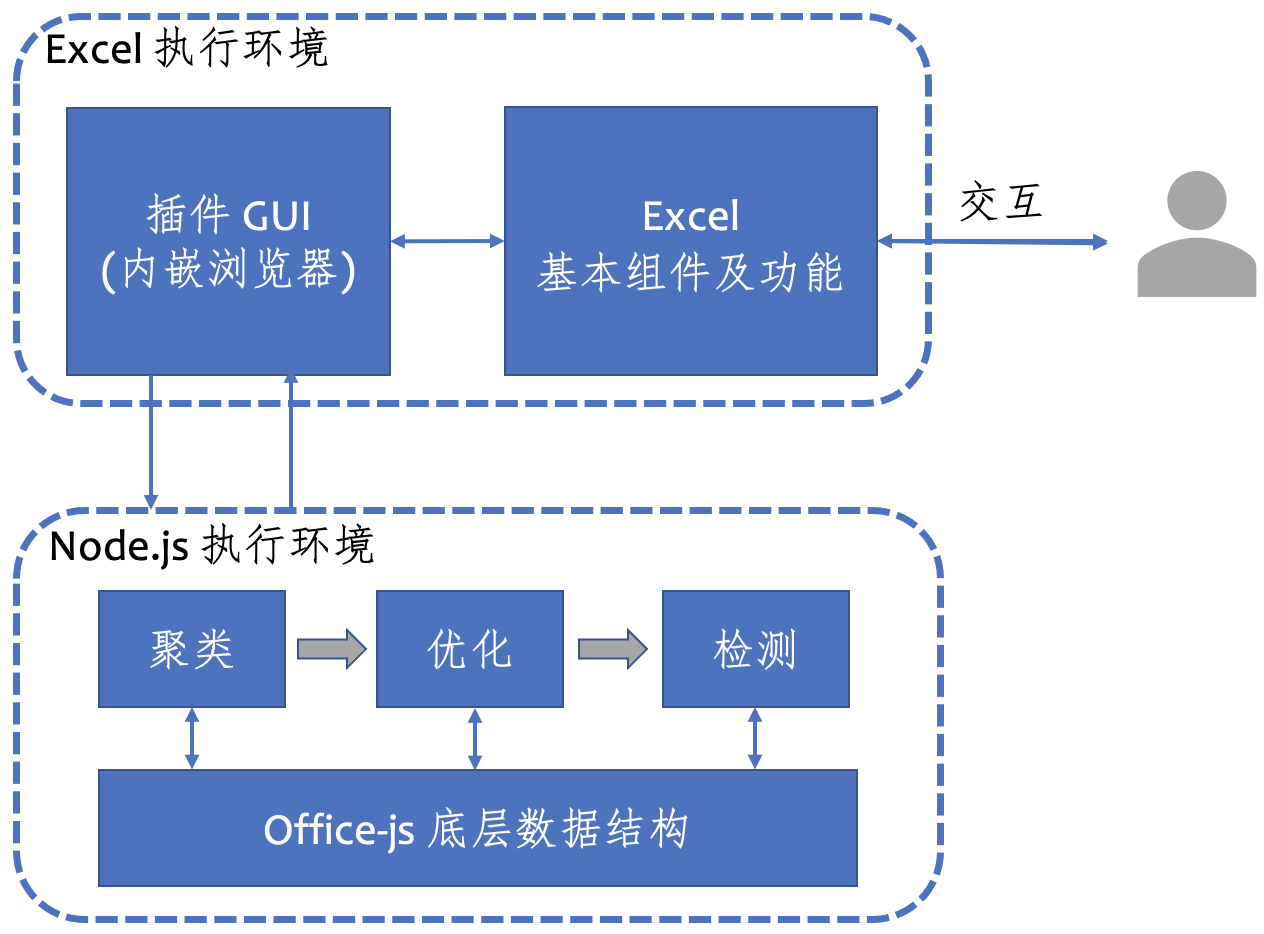
\includegraphics[width=0.8\textwidth]{figure/eg/eguard-framework.png}
    \caption{\eg 软件架构示意图}
    \label{figure-eg-framework}
\end{figure}
如图\ref{figure-eg-framework}所示,我们开发的 Excel 插件\eg 的整个运行框架包含两大部分:核心部分就是我们在 node.js 环境下使用 JavaScript 编写的所有核心算法模块;另外就是通过官方的 Office-js 框架实现 node.js 中算法代码和 Excel 中内嵌的插件系统进行异步通信,利用 ES6 中的 async/await 异步操作原语来实现数据交互和线程阻塞,本文的插件\eg 类似于服务器端代码,Excel 软件内如集成了插件系统,其功能类似于一个网页前端,通过 Office-js 框架定义好的通信协议进行数据传输。

插件\eg 的实现中主要包含三个核心模块:
\begin{itemize}
    \item \textbf{Excel中加载的插件界面模块}:界面模块主要包含对应于核心算法的三个模块,用户可以通过简单的交互界面,启动算法执行,并观察到每个算法模块的执行结果,并在 Excel 表格中看到对应的标注信息;
    \item \textbf{核心算法模块}:此模块主要包含方法设计部分提到的三个算法阶段,即单元格聚类,聚类优化和缺陷检测部分,每个算法部分由用户启动执行,执行完成后将额外的聚类或缺陷信息添加到底层数据结构中,并在插件界面中展示该部分的执行结果和细节信息,同时也对 Excel 表格中的单元格进行渲染,给用户比较好的直观提示;
    \item \textbf{底层数据结构模块}:在 Office-js 框架提供的获取 Excel 原数据的接口基础上,我们在原数据的基础上封装了算法实现和界面交互需要添加的属性,便于与另外两个模块进行交互。
\end{itemize}

我们简要介绍一下开发 Excel 插件的的单机测试流程:
\begin{itemize}
    \item 本工具使用浏览器测试,在https://onedrive.live.com/网址下打开或者新建一个电子表格;
    \item 在电子表格的菜单栏中依次选择“插入”、“Office 加载项”,并在弹出的“上传加载项”处填入对应的自己开发项目中的加载项清单,即对应的 manifest 文件中;
    \item 等待插件加载完成,打开浏览器自带的调试功能,开始进行界面和内部功能测试(以 Chrome 浏览器为例,测试日志一般会打印在 Console 窗口下),并进行对应的调试及编码工作。
\end{itemize}

接下来的两小节将结合具体的界面设计和使用展示来介绍\eg 。

\begin{figure}[tp]   
    \centering
    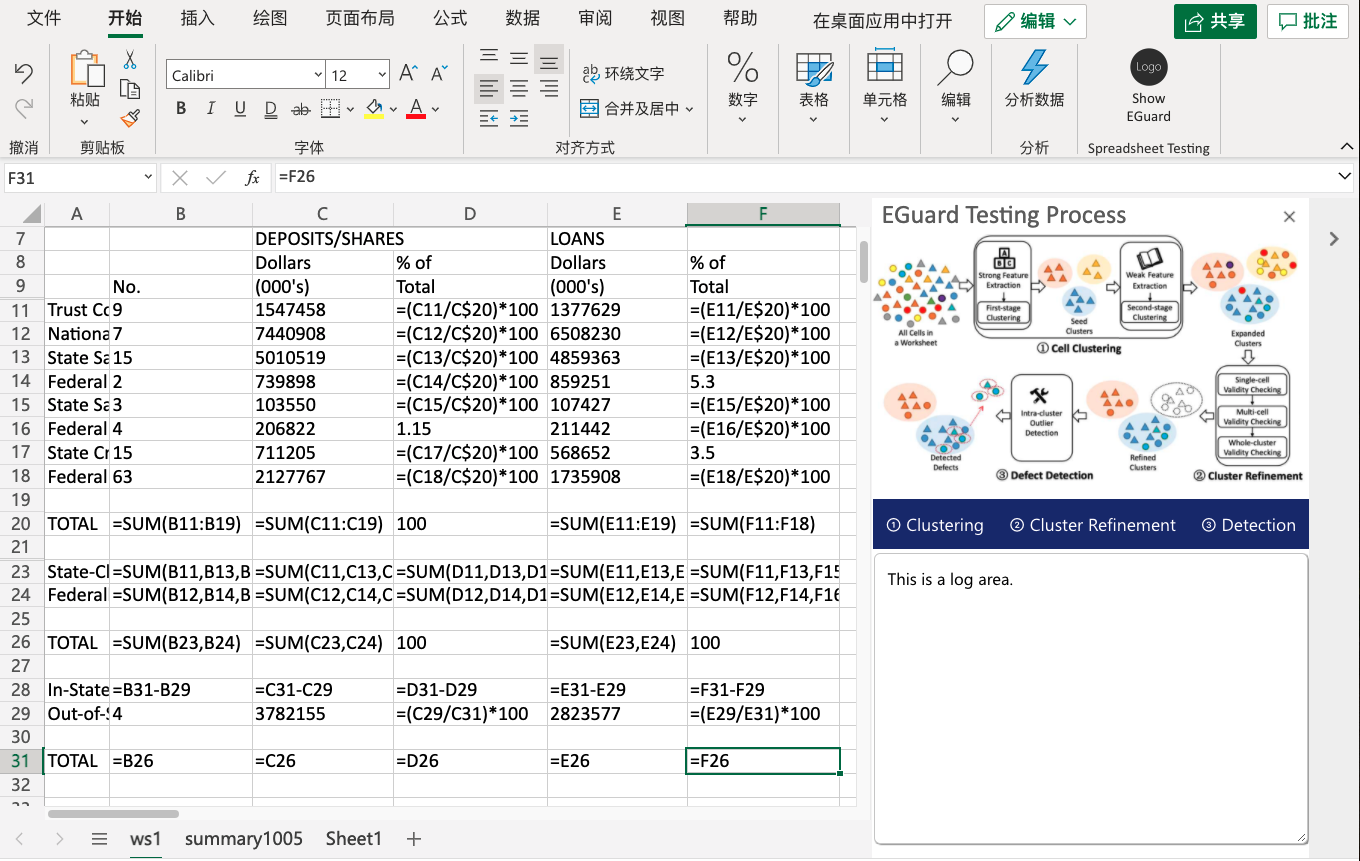
\includegraphics[width=\textwidth]{figure/eg/eguard-1.png}
    \caption{\eg 的插件布局}
    \label{figure-eg1}
\end{figure}
\begin{figure}[tbp]    
    \centering
    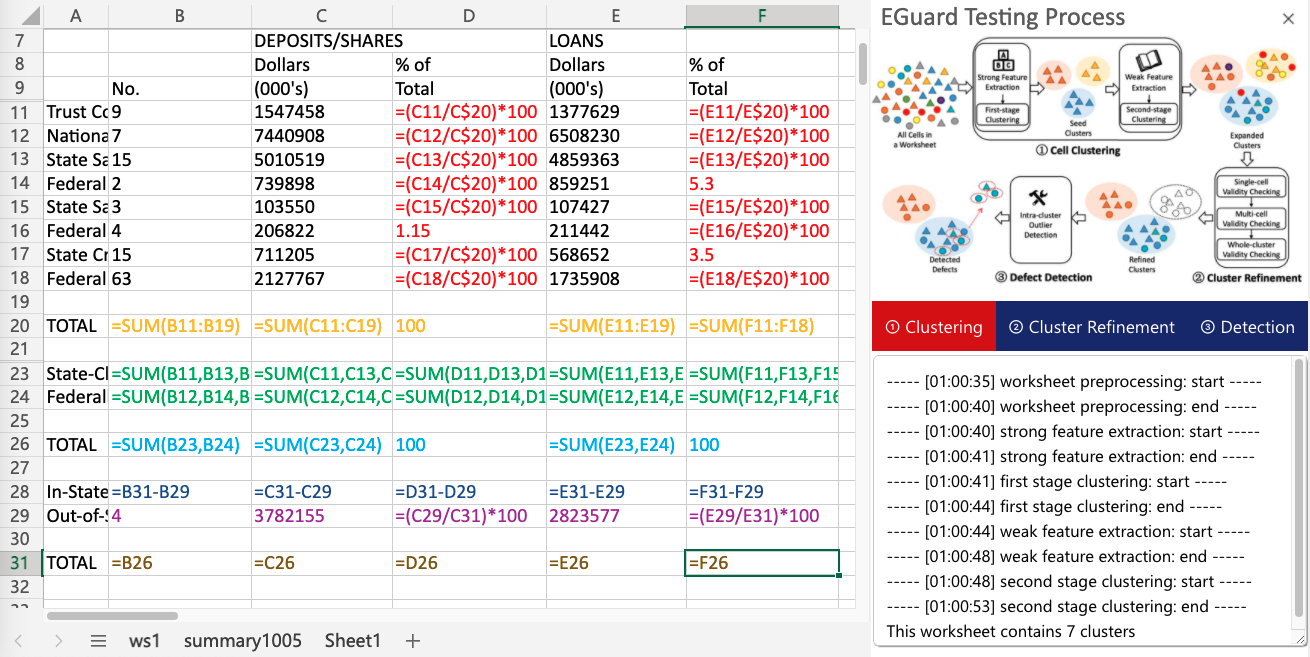
\includegraphics[width=\textwidth]{figure/eg/eguard-2.png}
    \caption{\eg 执行单元格聚类后的电子表格标记和执行信息输出}
    \label{figure-eg2}
\end{figure}
\begin{figure}[tbp]    
    \centering
    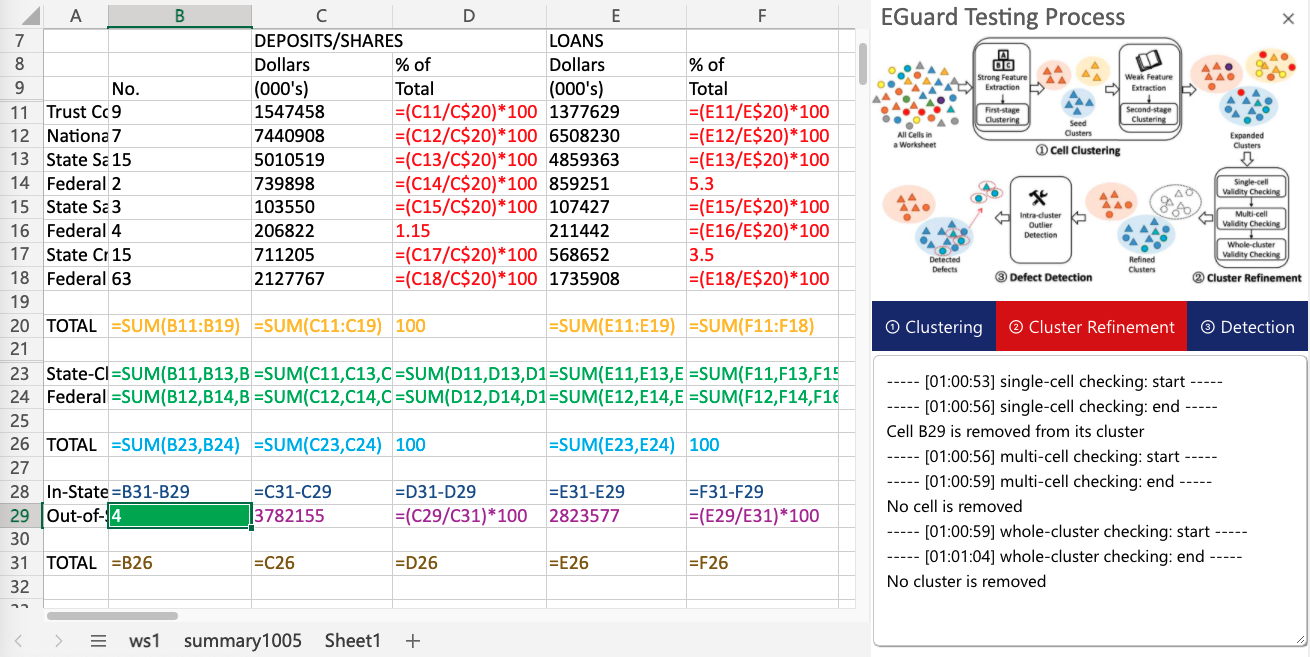
\includegraphics[width=\textwidth]{figure/eg/eguard-3.png}
    \caption{\eg 执行三个单元格检验方法后的电子表格标记和执行信息输出}
    \label{figure-eg3}
\end{figure}
\begin{figure}[tp]   
    \centering
    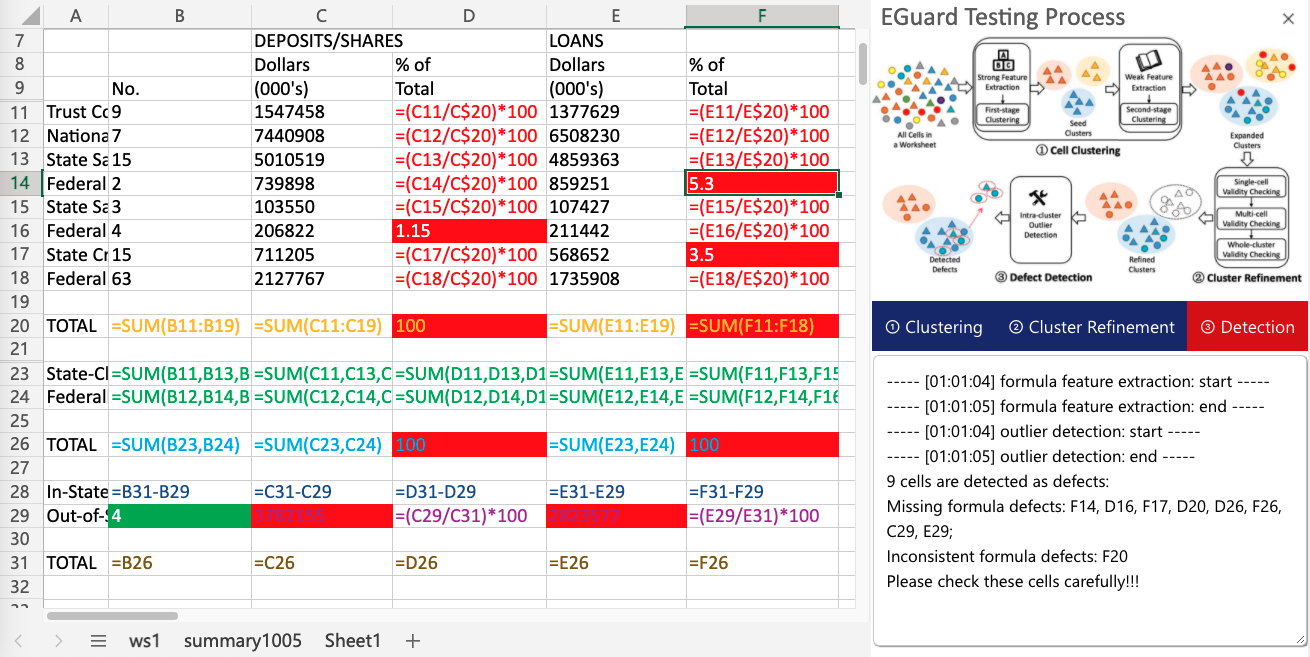
\includegraphics[width=\textwidth]{figure/eg/eguard-4.png}
    \caption{\eg 执行缺陷检测后的电子表格标记和执行信息输出}
    \label{figure-eg4}
\end{figure}

\subsection{界面设计}
如图\ref{figure-eg1}所示,在 Excel 软件中,从“插入”菜单栏选择“Office 加载项”按钮,然后选择本地的插件 \eg 进行加载。
加载完毕后,在“开始”菜单栏的最右侧会显示本文的插件工具图标,点击图标即显示出图\ref{figure-eg1}右侧的内嵌式网页,其标题是“EGuard Testing Process”。
整个内嵌式网页包含如下三个部分:

\begin{enumerate}
    \item 上方显示\eg 插件工具的执行流程图,方便终端用户对检测过程有一个直观感性的认识;
    \item 中间部分为一组选项卡,含有三个执行选项,依次为“\ding{172} Clustering”(两阶段的单元格聚类)、“\ding{173} Cluster Refinement”(基于有效性属性的检验) 和 “\ding{174} Detection”(缺陷检测);
    \item 下方是执行信息输出区域,显示执行的流程和对应的时间戳,以及一些帮助终端用户更好地理解检测结果的辅助信息。
\end{enumerate}

\subsection{使用展示}
接下来,我们结合一个具体的工作表来展示 \eg 的完整使用流程:
\begin{enumerate}
    \item 如图\ref{figure-eg1}所示,首先我们打开一个想要进行测试的 Excel 文件,并切换到想要进行测试的工作表,图中我们打开电子表格“illustrative\_example.xlsx”的工作表“ws1”,按上述方式加载 \eg 插件并在右侧打开嵌入式网页,为了方便观察聚类结果,我们把 Excel 的公式显示选项打开(默认显示 A1 表示法的公式形式);
    
    \item 如图\ref{figure-eg2}所示,点击“\ding{172} Clustering”选项卡按钮,即开始对当前工作表执行强弱特征抽取和两阶段的单元格聚类任务,在插件下方可以看到具体的执行流程包括每个子任务对应的执行时长和一些辅助用户理解的信息。如图所示,最终通过两阶段聚类检测到了 7 个单元格类,并在工作表中用不同的字体颜色标注出来;
    
    \item 如图\ref{figure-eg3}所示,点击“\ding{173} Cluster Refinement”选项卡按钮,即在两阶段聚类的基础上执行针对本文提出的\wa 方法,即第四章描述的 3 种基于有效性属性的检验方法。在当前示例中,依据单个单元格有效性属性检验结果,将单元格 B29 从原先的单元格类 \{B29,C29,D29,E29,F29\} 中移除,因为该单元格并不具备和其他单元格类似的除法运算语义,即如果 B29 具有类似公式,则会显示为=(A29$/$A31)$*$100,但 A29 和 A31 都是字符串单元格,无法进行数值运算。从表中可观察到,被移除的单元格会用绿色背景和白色字体标注出来;
    
    \item 如图\ref{figure-eg4}所示,点击“\ding{174} Detection”选项卡按钮,即在聚类和检验的基础上,进行类内缺陷检测,在当前工作表中,分别从 4 个单元格类中检测出 9 个有缺陷的单元格,其中 8 个为含有常量替换的公式缺陷的单元格,即 F14、D16、F17、D20、D26、F26、C29 和 E29,以及 1 个引用替换的公式缺陷的单元格 F20。从工作表中可观察到,有缺陷的单元格会用红色背景标注出来,如果原来该单元格就是红色字体,为显示结果清晰,则相应改为白色字体,如单元格 D16;
    
    \item 最后,用户可以结合工作表中的标注信息(字体颜色和背景色)和插件下方的日志信息,对工具标记为有公式缺陷的单元格进行检查和修订。
\end{enumerate}


